\section{Signalweg}
\begin{center}
    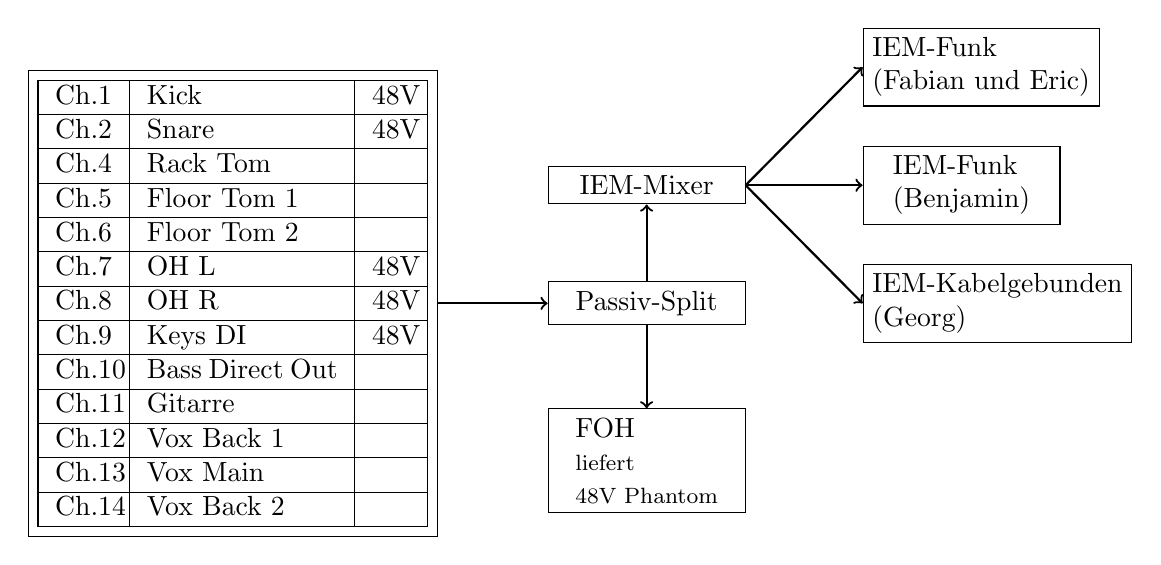
\begin{tikzpicture}
    %Place table node
    \node[draw, rectangle, minimum width=5cm, minimum height=5cm, align=center] (table) at (0,0) {\begin{tabular}{|p{0.06\textwidth}|p{0.2\textwidth}|p{0.04\textwidth}|}
        \hline
        Ch.1 & Kick & 48V \\
        \hline
        Ch.2 & Snare & 48V \\
        \hline
        Ch.4 & Rack Tom & \\
        \hline
        Ch.5 & Floor Tom 1 & \\
        \hline
        Ch.6 & Floor Tom 2 & \\
        \hline
        Ch.7 & OH L & 48V \\
        \hline
        Ch.8 & OH R & 48V \\
        \hline
        Ch.9 & Keys DI & 48V \\
        \hline
        Ch.10 & Bass Direct Out & \\
        \hline
        Ch.11 & Gitarre & \\
        \hline
        Ch.12 & Vox Back 1 & \\
        \hline
        Ch.13 & Vox Main & \\
        \hline
        Ch.14 & Vox Back 2 & \\
        \hline
    \end{tabular}};
    
    %Place passive-split node
    \node[draw, rectangle, minimum width=2.5cm, align=left, anchor=west] (split) at (4,0) {Passiv-Split};

    %Place FOH node
    \node[draw, rectangle, minimum width=2.5cm, align=left, anchor=west] (foh) at (4,-2) {FOH \\ \footnotesize liefert \\ \footnotesize 48V Phantom};

    %Place IEM-Mixer node
    \node[draw, rectangle, minimum width=2.5cm, align=left, anchor=west] (iem-mixer) at (4,1.5) {IEM-Mixer};

    %Place IEM-Fabian-Eric Node
    \node[draw, rectangle, minimum width=2.5cm, align=left, anchor=west] (fabian-eric) at (8,3) {IEM-Funk \\ (Fabian und Eric)};

    %Place IEM-Benjamin Node
    \node[draw, rectangle, minimum width=2.5cm, align=left, anchor=west] (benjamin) at (8,1.5) {IEM-Funk \\ (Benjamin)};

    %Place IEM-Georg Node
    \node[draw, rectangle, minimum width=2.5cm, align=left, anchor=west] (georg) at (8,0) {IEM-Kabelgebunden \\ (Georg)};
    
    %Draw arrows
    \draw[->, thick] (table.east) -- (split.west);
    \draw[->, thick] (split.north) -- (iem-mixer.south);
    \draw[->, thick] (split.south) -- (foh.north);
    \draw[->, thick] (iem-mixer.east) -- (fabian-eric.west);
    \draw[->, thick] (iem-mixer.east) -- (benjamin.west);
    \draw[->, thick] (iem-mixer.east) -- (georg.west);
\end{tikzpicture}
\end{center}